\documentclass[11pt]{article}

% parameters are fairly self-explanatory here, thankfully
\usepackage[width=7in,height=9.5in,top=0.75in,centering]{geometry}

% for math-ing
\usepackage{amsmath}
\usepackage{amssymb}

%%%%%% tables %%%%%%%%

\usepackage{array}
\renewcommand{\arraystretch}{1.5}
\setlength{\tabcolsep}{8pt}

%%%%%% plotting %%%%%%

\usepackage[dvipsnames]{xcolor}
\usepackage{tikz}
\usepackage{pgfplots}

\pgfplotsset{every axis/.append style={
                    axis x line=middle,    % put the x axis in the middle
                    axis y line=middle,    % put the y axis in the middle
                    axis line style={<->,color=black}, % arrows on the axis
                    xlabel={$x$},          % default put x on x-axis
                    ylabel={$y$},          % default put y on y-axis
            }}
            
 \pgfplotsset{compat=1.14} % sometimes, everything falls apart without this
 
 %\usepgfplotslibrary{fillbetween} %for shading between curves

%%%%%% commands %%%%%%

% exam heading; course name is first argument, exam information is second argument
\newcommand{\Heading}[2]{
    \fbox{
        {\Large\textbf{#1}}
        }
    \hfill
    \fbox{
        \begin{minipage}{0.2\textwidth}
            \begin{center}
            \textbf{#2}
            \end{center}
        \end{minipage}
    }
    \par\vspace{0.1in}}

% for being lazy while beautifying integrals
\newcommand{\dint}{\displaystyle\int}

% for being lazy while beautifying limits
\newcommand{\dlim}{\displaystyle\lim}

%%%%%% stuff %%%%%%

\usepackage{fancyhdr}

%\setcounter{page}{0} % first page is page 0

\parindent0pt % no indent

\fboxsep=0.25cm % little space in fbox border

%%%%%% BEGIN! %%%%%%%

\begin{document}

\pagestyle{fancy}

% record goals here to create sense of transparency

\fancyhead[c]{%
  \ifcase\value{page}
  % empty test for page = 0
  % \or {}% 
  % \or
  % \or {\bf\color{ProcessBlue} F2: Exponentials \& Log Functions}% page=1
  % \or {\bf\color{ForestGreen} D2: Compute Derivatives}% page = 2
  % \or {\bf\color{ForestGreen} D3: Derivatives of Basic Functions}% page = 3
  \or {\bf\color{RedOrange} A1: Derivatives and Graphing}% page = 4
  \or
  \or {\bf\color{RedOrange} A2: Local and Absolute Extreme Values}% page = 5
  \or {\bf\color{RedOrange} A3: Applied Optimization}% page = 7
  \or {\bf\color{Fuchsia} I1: Meaning of an Integral}% page = 6
  \or {\bf\color{Fuchsia} I2: Properties of Definite Integrals}% page = 8
  \or
  \else
  % Empty chead here!
  \fi
}

% \thispagestyle{empty} % don't display that this is page 0

\Heading{MATH 1210}{Review Session 3\\
A1--A3, I1--I2
Spring 2026\\
Section 930}

\vspace{0.1in}

\textbf{Name} \hrulefill
% \newpage%
%%%%%%%%%


\begin{enumerate}

%%%%%%%%%%%%%%%%%%%%%%%%%%%%%%%%%%%%%%%%%%%%%%%%%%%%%
%%%%%%%%%%% BEGIN PROBLEM F2 %%%%%%%%%%%%%%%%%%%%%%%%
%%%%%%%%%%%%%%%%%%%%%%%%%%%%%%%%%%%%%%%%%%%%%%%%%%%%%

% \item[\textbf{F2.}]
% For this question, you are not required to compute any powers of constants or logarithms.
% For example, if your final answer includes $2^3$ or $\log_3(6)$, you can leave it as is.

% \begin{enumerate}
% \item
% Simplify the expression below as much as possible so that the final result contains \textbf{only positive exponents}.
% \begin{enumerate}
% \item
% $\left(\dfrac{\sqrt[3]{25} \ a^{-3/4} \ b^{-2/3}}{\sqrt{4} \ a^{-1/2} \ b^{2/3}}\right)^3$
% \vfill
% \item
% $\left(\dfrac{49 \ m^{-1/2} \ n^{-3/5}}{7^2 \ m^{-1/4} \ n^{-1/5}}\right)^{11}$
% \end{enumerate}
% \vfill

% \item Solve the following equation for $x$. 
% \begin{enumerate}
% \item
% $5^{2x} + 2\cdot 5^x - 3 = 0$
% \vfill
% \item
% $\log_{5}(x) - \log_{5}(x^3-7x^2) + \log_{5}(x - 7) = 3$
% \end{enumerate}
% ~~\vfill
% \end{enumerate}

% \newpage


%%%%%%%%%%%%%%%%%%%%%%%%%%%%%%%%%%%%%%%%%%%%%%%%%%%%%
%%%%%%%%%%% END PROBLEM F2 %%%%%%%%%%%%%%%%%%%%%%%%%%
%%%%%%%%%%%%%%%%%%%%%%%%%%%%%%%%%%%%%%%%%%%%%%%%%%%%%



%%%%%%%%%%%%%%%%%%%%%%%%%%%%%%%%%%%%%%%%%%%%%%%%%%%%%
%%%%%%%%%%% BEGIN PROBLEM D2/D3 %%%%%%%%%%%%%%%%%%%%%%%%
%%%%%%%%%%%%%%%%%%%%%%%%%%%%%%%%%%%%%%%%%%%%%%%%%%%%%

% \item[\textbf{D2/D3.}]
% Write down the derivatives of the following functions.
% No need to simplify.
% \begin{enumerate}

% \item $\displaystyle \frac{d}{dx}\left[ \frac{\ln(x)}{x^3} \right]$
% \vfill
% \item $\displaystyle \frac{d}{dx}\left[ \frac{x e^{x^2}}{x^2+1} \right]$
% \vfill
% \item $\displaystyle \frac{d}{dx}\left[ (x^3+1)e^{-2x}\right]$
% \vfill
% \end{enumerate}

% \newpage


%%%%%%%%%%%%%%%%%%%%%%%%%%%%%%%%%%%%%%%%%%%%%%%%%%%%%
%%%%%%%%%%% END PROBLEM D2/D3 %%%%%%%%%%%%%%%%%%%%%%%%%%
%%%%%%%%%%%%%%%%%%%%%%%%%%%%%%%%%%%%%%%%%%%%%%%%%%%%%


%%%%%%%%%%%%%%%%%%%%%%%%%%%%%%%%%%%%%%%%%%%%%%%%%%%%%
%%%%%%%%%%% BEGIN PROBLEM D2/D3 %%%%%%%%%%%%%%%%%%%%%%%%
%%%%%%%%%%%%%%%%%%%%%%%%%%%%%%%%%%%%%%%%%%%%%%%%%%%%%

% \item[\textbf{D2/D3.}]
% Write down the derivative of the following function.
% No need to simplify.
% \[\displaystyle \frac{d}{dx}\left[ \ln\left(\frac{(x^2+3)e^{x}}{x} \right)\right]\]
% \vfill


% \newpage


%%%%%%%%%%%%%%%%%%%%%%%%%%%%%%%%%%%%%%%%%%%%%%%%%%%%%
%%%%%%%%%%% END PROBLEM D2/D3 %%%%%%%%%%%%%%%%%%%%%%%%%%
%%%%%%%%%%%%%%%%%%%%%%%%%%%%%%%%%%%%%%%%%%%%%%%%%%%%%

%%%%%%%%%%%%%%%%%%%%%%%%%%%%%%%%%%%%%%%%%%%%%%%%%%%%%
%%%%%%%%%%% BEGIN PROBLEM A1 %%%%%%%%%%%%%%%%%%%%%%%%
%%%%%%%%%%%%%%%%%%%%%%%%%%%%%%%%%%%%%%%%%%%%%%%%%%%%%

\item[\textbf{A1.}]
Consider the following function:
$f(x) = \sqrt{x}\left(x - 4\right)$.
\begin{enumerate}
\item
What is the domain of $f(x)$?
\item
At what $x$-values does $f(x)$ have its critical numbers?
\vfill
\item 
On what interval(s) is $f(x)$ concave up? On what interval(s) is $f(x)$ concave down?
\vfill
\item
At what $x$-values does $f(x)$ have its inflection points?
\vfill
\end{enumerate}
\newpage


%%%%%%%%%%%%%%%%%%%%%%%%%%%%%%%%%%%%%%%%%%%%%%%%%%%%%
%%%%%%%%%%% END PROBLEM A1 %%%%%%%%%%%%%%%%%%%%%%%%%%
%%%%%%%%%%%%%%%%%%%%%%%%%%%%%%%%%%%%%%%%%%%%%%%%%%%%%

\begin{itemize}
\item\textbf{First Derivative Test.}
Suppose that $c$ is a
\textbf{critical number}
of a continuous function $f$.
\begin{enumerate}
\item
If $f'$ changes from
\textbf{positive}
to
\textbf{negative}
at $c$, then $f$ has a
\textbf{local maximum} at $c$.
\item
If $f'$ changes from
\textbf{negative}
to
\textbf{positive}
at $c$, then $f$ has a
\textbf{local minimum}
at $c$.
\item
If $f'$ does not change sign at $c$,
then $f$ has
\textbf{neither local maximum, nor local minimum}
at $c$.
\end{enumerate}
\vfill
\item\textbf{Second Derivative Test.}
Suppose $f''$ is continuous near a critical number $x=c$.
\begin{enumerate}
\item
If \textbf{$f^{\prime}(c)=0$ and $f^{\prime\prime}(c)<0$}
then we have a
\textbf{local maximum at $x=c$}.
\item
If \textbf{$f^{\prime}(c)=0$ and $f^{\prime\prime}(c)>0$}
then we have a
\textbf{local minimum at $x=c$}.
\item
If \textbf{$f^{\prime}(c)$ DNE,
$f^{\prime\prime}(c)=0$, or
$f^{\prime\prime}(c)$ DNE}
then we cannot use the Second Derivative Test\\
(i.e. the \textbf{test is inconclusive}).
\end{enumerate}
\vfill
\item
\textbf{Closed Interval Method.}
To find the absolute maximum value and absolute minimum value of a continuous function $f$ on the closed interval $[a, b]$, do the following:
\smallskip

\begin{minipage}{0.75\textwidth}
\begin{enumerate}
\item  Find the critical numbers $c_1, c_2, \ldots, c_n$ of $f$ that lie in $(a, b)$.
\item  Find the value of $f$ at each critical number {\em and} at the endpoints


\item  The largest value from (b)  will be the absolute maximum value of $f$ on $[a, b]$ and the smallest value from (b) will be the absolute minimum value of $f$ on $[a, b]$. 
\end{enumerate}
\end{minipage}
%
\hfill
%
\begin{minipage}{0.2\textwidth}
\begin{center}
\begin{tabular}{|c|c|}
\hline 
$x$ & $f(x)$\tabularnewline
\hline 
\hline 
$a$ & $f(a)$\tabularnewline
\hline 
$b$ & $f(b)$\tabularnewline
\hline 
$c_1$ & $f(c_1)$\tabularnewline
\hline 
$c_2$ & $f(c_2)$\tabularnewline
\hline 
$\vdots$ &$\vdots $\tabularnewline
\hline 
$c_n$ & $f(c_n)$\tabularnewline
\hline 
\end{tabular}
\end{center}
\end{minipage}
\vfill
\item
\textbf{First Derivative Test for Absolute Extrema.}
Suppose that $c$ is a critical number of a continuous function $f$ defined on an interval $I$.
    \begin{itemize}
    \item {\bf If} the sign of $f'$ changes from positive ($+$) to negative ($-$) at $c$ {\bf and} $c$ is the only critical number where $f^{\prime}$ changes sign on $I$
    %\emph{and} if $c$ is the only $x$-value in $I$ at which $f$ changes sign, 
    {\bf then} $f(c)$ is the absolute maximum value of $f$ on $I$.
    \item {\bf If} the sign of $f'$ changes from negative ($-$) to positive ($+$) at $c$ {\bf and} $c$ is the only critical number where $f^{\prime}$ changes sign on $I$
    % \emph{and} if $c$ is the only $x$-value in $I$ at which $f$ changes sign, 
    {\bf then} $f(c)$ is the absolute minimum value of $f$ on $I$.\\
    \end{itemize}
\end{itemize}
\newpage

\item[\textbf{A2.}]
Let $f(x)=x+\dfrac4x$. Additionally, note that $f'(x)=1-\dfrac4{x^2}$ and $f''(x)=\dfrac{8}{x^3}$.
    \begin{itemize}
    \item[(a)] Find all critical numbers of $f$.
        
        \vfill
        \vfill
        
    \item[(b)] For each critical number, determine whether a local maximum, a local minimum, or neither occurs at the critical number.

        \vfill
        \vfill
        \vfill

    \item[(c)] Identify the absolute extrema of $f$ on the interval $\left[-8,-1\right]$.

        \vfill
        \vfill
    
    \end{itemize}

\newpage


\item[\textbf{A3.}]
The top and bottom margins of a rectangular poster are $15$ cm and the side margins are each $10$ cm. If the area of printed material on the poster is fixed at $2400$ cm$^2$, find the dimensions of the poster with the smallest area.
\newpage


\item[\textbf{I1.}]
The drawing below represents a loaf of bread with a cut shown $l$ inches from the left-hand end of the bread. Let $A(l)$ represent the rate of change of the volume of bread to the left of the cut with respect to $l$.

\begin{center}
\includegraphics[width=0.6\textwidth]{images/CCIbread.PNG}\end{center}
    
    You may assume $A(l)$ is measured in cubic inches of bread per 1 inch slice. 
    
    \begin{enumerate}
    \item What does $\displaystyle\int_0^4 A(l)\,dl$ represent? What are its units?
    
        \vfill

    \,\hfill units: \rule[-8pt]{3in}{0.4pt}\\[0.1in]
    

    \item If the loaf were 15 inches long and the cut in the image above were at $l=12$ inches, then which {\bf two} of the following integrals are largest? {\bf Circle two.}\\

    \,\hfill
    \fbox{A} $\displaystyle\int_0^3 A(l)\,dl$
    \hfill
    \fbox{B} $\displaystyle\int_3^6 A(l)\,dl$
    \hfill
    \fbox{C} $\displaystyle\int_6^9 A(l)\,dl$
    \hfill
    \fbox{D} $\displaystyle\int_9^{12} A(l)\,dl$
    \hfill
    \fbox{E} $\displaystyle\int_{12}^{15} A(l)\,dl$
    \hfill\,\\[0.1in]
\vfill
    \end{enumerate}

\newpage


\item[\textbf{I2.}]
The graph of the function $f$ consists of a line segment followed by a quarter circle, followed by another line segment, and is given below:

\begin{center}
        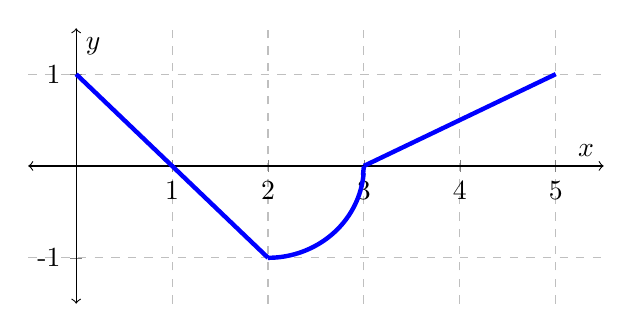
\begin{tikzpicture}
              \begin{axis}[
            %    axis y line = left,
            %    axis x line = bottom,
                xlabel = {$x$},
                ylabel = {$y$},
                ytick       = {-1,1,2,3,4,5},
                yticklabels = {-1,1,2,3,4,5},
                xtick       = {1,2,3,4,5},
                xticklabels = {1,2,3,4,5},
                samples     = 320,
                %domain      = 0:4,
                %restrict y to domain=-5:5,
                ymin = -1.5, ymax = 1.5,
                xmin = -0.5, xmax = 5.5,
                width=3.5in,height=2in,
                grid=both, grid style=dashed
              ]
             %
             \addplot[domain=2:3,blue, ultra thick, mark=none, smooth] {-(1-(x-2)^2)^(1/2)};
             \draw[ultra thick,blue] (2.99,-0.1) -- (3,0);
             \draw[ultra thick,blue] (0,1) -- (2,-1);
             \draw[ultra thick,blue] (3,0) -- (5,1);
             %
             \end{axis}
        \end{tikzpicture}    
    \end{center}

    \begin{itemize}

    \item[(a)]
    Find $\displaystyle\int_1^5 f(x)\,dx$.
        \vfill
        
    \item[(b)] Suppose for some function $g$ that $\displaystyle\int_0^3 (4f(x)+g(x))\,dx=\pi$ and $\displaystyle\int_3^5 g(x)\,dx=-\pi$. 
        \begin{itemize}
        \item[i.] Find $\displaystyle\int_0^3 g(x)\,dx$.
        \vfill

        \item[ii.] Find $\displaystyle\int_0^5 g(x)\,dx$.
        \vfill
        \end{itemize}
        
    \end{itemize}


\end{enumerate}
\end{document}